\documentclass{standalone}
\usepackage{mintikz}

\def\A{0.25}
\def\Q{6}
\def\wo{1e3}
\def\fo{\wo/2*pi}

\begin{document}
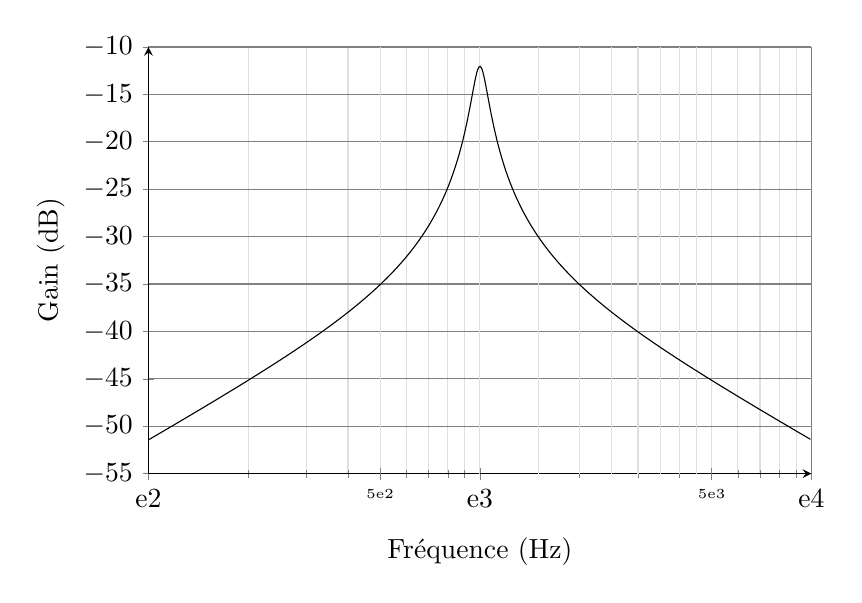
\begin{tikzpicture}[]
    \begin{semilogxaxis}[
        xmin=1e2, xmax=1e4,
        xticklabels={\num{e2}, \num{e3}, \num{e4}},
        extra x ticks={5e2, 5e3},
        extra x tick labels={\num{5e2}, \num{5e3}},
        extra x tick style={grid=minor, grid style={gray!25}, font=\tiny},
        ymin=-55, ymax=-10,
        ytick={-55, -50, ..., -10},
        xlabel=Fr\'equence (Hz), ylabel=Gain (dB),
        axis lines=left,
        grid=both,
        minor grid style={gray!25},
        major grid style={black!50},
        width=10cm,
        height=7cm,
        clip=true]
        \addplot[
        domain=1e2:1e4,
        smooth,
        samples=500,
        black]
        {20*log10(\A/(sqrt(1 + \Q^2*(\x/\fo - \fo/\x)^2)))};
    \end{semilogxaxis}
\end{tikzpicture}
\end{document}
